\documentclass[11pt]{article}

\usepackage[margin=1.1in]{geometry}
\usepackage{amsmath,amssymb}
\usepackage{graphicx}
\usepackage{booktabs}
\usepackage{caption}
\usepackage{enumitem}
\usepackage{xcolor}
\usepackage[colorlinks=true,linkcolor=blue!50!black,citecolor=blue!50!black,urlcolor=blue!50!black]{hyperref}
\usepackage{natbib}

\title{Sparse Bayesian Cross-Sectional Return Forecasting with\\
Correlation-Block Factors: A Real-Time-Valid Test\\
Against the M6 Financial Forecasting Competition}
\author{Ian Johnston}
\date{\today}

\begin{document}
\maketitle

\begin{abstract}
\noindent
We propose a hierarchical Bayesian model for cross-sectional return
forecasting that addresses a specific, common obstacle in factor-based
investing: a candidate universe of assets is large and highly
inter-correlated, so naive regression either wastes power spreading
credit across redundant, co-moving assets or overstates confidence in
whichever one happens to enter the model first. The model groups
correlated assets into blocks, summarizes each block by a single latent
factor, and then performs Bayesian spike-and-slab variable selection on
the resulting block factors, with the prior probability that a block
matters informed by an auditable sector-relevance score rather than left
uniform. We evaluate the resulting strategy against the M6 Financial
Forecasting Competition, a real, independently judged, 100-asset
contest with published results for 163 competing teams, under a single
governing constraint: every parameter used in period $p$ must be
computable from information available strictly before period $p$ began.
Enforcing that constraint required finding and fixing three distinct,
individually plausible-looking sources of look-ahead bias, which we
present as a general checklist. The resulting strategy, run causally
through the real 2022 competition window, would have placed in the top
2\% of the field on the competition's joint ranking, against an actual
historical result (the author's own real submissions that year) that
placed in the bottom third. Extended out-of-sample through three further
years (2023--2025) never used to design any part of the model, the
result holds and strengthens: the forecast beats the naive benchmark in
40 of 48 periods ($p<0.0001$) and the resulting portfolio's information
ratio is positive in 30 of 48 ($p=0.04$).
\end{abstract}

% ============================================================
\section{Introduction}
% ============================================================

Cross-sectional return forecasting --- ranking a fixed universe of assets
by expected relative performance over some future window --- runs into
the same obstacle almost regardless of universe: the candidate predictors
are numerous and highly correlated with one another. A momentum signal on
one technology stock is not independent information from the same signal
on five other technology stocks; a naive regression across all of them
either dilutes real signal across redundant, co-moving variables, or
overfits by handing all the credit to whichever one entered the model
first. The empirical asset-pricing literature has approached this problem
from several angles --- dimension reduction via latent factors
\citep{kellypruittsu2020}, penalized regression across the ``characteristics
zoo'' \citep{degroot2018}, and Bayesian model averaging over predictor
uncertainty \citep{avramov2002}. This paper contributes a specific
architecture to that list: a two-stage \emph{decorrelate, then select}
model that groups correlated assets into blocks, extracts one latent
factor per block, and performs Bayesian spike-and-slab selection on the
resulting factors with an externally informed, auditable prior on which
blocks are likely to matter.

We test the model not on a synthetic or in-sample benchmark, but against
the M6 Financial Forecasting Competition \citep{makridakis2024}: a real,
independently run, crowd-benchmarked contest with a fixed 100-asset
universe, a public scoring methodology, and published results for every
one of 163 real competing teams. This is a meaningfully harder bar than
most backtests clear. In the actual competition, only 23.3\% of real
teams beat the naive uniform-probability benchmark on average forecast
accuracy, and only 8.6\% beat it with statistical significance --- a
useful reminder of how little exploitable structure typically survives
contact with live, adversarial evaluation.

Testing against a real competition, rather than an in-sample historical
period, imposed a discipline that turned out to matter more than any
single modeling choice: \emph{every parameter or design decision used to
produce period $p$'s forecast must be computable using only information
available strictly before period $p$ began.} This sounds obvious stated
plainly, but an earlier version of this pipeline violated it three
separate times, in three different and individually unremarkable-looking
ways, each of which inflated the backtest's apparent performance until
caught. Section \ref{sec:realtime} documents all three as a general
checklist, because we believe the pattern is more broadly useful to a
practitioner than the specific fixes.

\subsection*{Relation to prior work on M6 specifically}
The M6 competition has already produced at least one directly comparable
result: \citet{weitzenfeld2025} won the competition's forecasting
(accuracy) track with a Bayesian dynamic factor model with time-varying
heteroskedasticity, fit by Markov chain Monte Carlo, that also uses
hierarchical shrinkage in place of a hand-picked cross-sectional variance
structure. That result is good independent evidence that Bayesian
hierarchical factor models are a genuinely strong approach to this
specific problem, not an artifact of any one author's design choices.
This paper's architecture differs in two respects worth naming plainly.
First, it performs explicit \emph{group-level model selection}
(spike-and-slab over blocks, so which blocks matter is itself inferred
and can vary sparsely from asset to asset) rather than a dense factor
model with all blocks always contributing. Second, its group-inclusion
prior is informed by an external, auditable relevance judgment (sector
adjacency) rather than estimated symmetrically from the data alone. We
see these as complementary design choices, not a claim of superiority ---
Weitzenfeld's model won the forecasting track outright, and our own
result is stronger on the investment-decision (portfolio) side than on
forecast accuracy per se, which Section \ref{sec:results} reports plainly
rather than downplaying.

\subsection*{Contributions}
\begin{itemize}[leftmargin=1.4em,itemsep=1pt]
  \item A hierarchical spike-and-slab block-factor architecture for
  cross-sectional forecasting, with an externally informed group-inclusion
  prior (Section \ref{sec:model}).
  \item A general, three-item checklist for eliminating look-ahead bias in
  walk-forward financial backtests, developed by finding and fixing three
  real instances of it in this pipeline (Section \ref{sec:realtime}).
  \item A full, causally valid backtest against the real M6 2022
  competition, with placement against the actual 163-team leaderboard
  (Section \ref{sec:results}).
  \item An out-of-sample extension through three further years never used
  in any design decision, showing the result holds and strengthens under
  a larger sample (Section \ref{sec:results}).
\end{itemize}

% ============================================================
\section{Model: Correlation-Block Factors with an Informed Selection Prior}
\label{sec:model}
% ============================================================

The model is built for a specific, common situation: forecasting one
target asset's return from a large panel of other candidate predictor
assets that are themselves highly inter-correlated. It proceeds in two
stages, deliberately kept separate.

\subsection{Stage 1: decorrelate via block factors}
The $n-1$ non-target assets in a universe of $n$ are grouped into blocks
by a correlation threshold on trailing returns, so that assets within a
block are strongly co-moving and assets in different blocks are
comparatively independent. Within each block, a one-factor Gaussian model
(a probabilistic-PCA-style construction) extracts a single latent factor
summarizing the block's shared movement, closed-form and non-iterative
under a Gaussian-identity link. This stage is entirely
target-independent: block formation and factor extraction use only the
predictor panel's own correlation structure, never the return being
forecast, so the same block factors can be reused as candidate predictors
for every target asset in the universe.

\subsection{Stage 2: Bayesian spike-and-slab selection with an informed prior}
The target asset's own historical return is then regressed on the block
factors from Stage 1 via Bayesian spike-and-slab variable selection
\citep{mitchellbeauchamp1988,georgemcculloch1993,ishwaranrao2005}. Each block
$j$ carries a binary inclusion indicator $\gamma_j \in \{0,1\}$ with slab
coefficient $\beta_j$ under $\gamma_j=1$ and a point mass at zero under
$\gamma_j=0$; the joint posterior over $(\gamma,\beta)$ is sampled by
Gibbs sampling, which is fully conjugate for a continuous (Gaussian)
outcome and requires no tuning of an approximate gradient step. The
detail that matters most for the exercise in this paper is where the
prior inclusion probability $\pi_j = P(\gamma_j = 1)$ comes from: rather
than a single uniform value shared across all blocks, $\pi_j$ is set by
an auditable relevance score between the target asset's own sector and
the sector composition of block $j$'s member assets (Table
\ref{tab:relevance}). This does the same conceptual job as an
economically motivated exclusion restriction in a standard regression ---
it does not force any block in or out, but it tilts the posterior toward
finding a same-sector block relevant and away from a spuriously
correlated but economically unconnected one, without ever preventing the
data from overriding that tilt when the evidence is strong enough.

\begin{table}[htbp]
\centering
\begin{tabular}{@{}lc@{}}
\toprule
Relationship of a candidate block's sector to the target's own sector & Prior relevance score \\
\midrule
Same sector                                   & 5.0 \\
Adjacent sector (e.g.\ Technology $\leftrightarrow$ Communication Services) & 3.0 \\
Broad-market (diversified index exposure)     & 2.0 \\
International / regional                      & 1.0 \\
Unrelated sector                               & 0.5 \\
Fixed income, commodities, or volatility products & 0.05 \\
\bottomrule
\end{tabular}
\caption{The sector-relevance scoring table used to set each block's prior
inclusion probability $\pi_j$ in Application 1 (Section
\ref{sec:applications}). This table encodes a real assumption --- that
fixed-income and commodity exposure is usually irrelevant to a single
equity or equity-ETF target --- which is appropriate here but, as Section
\ref{sec:applications} notes, is the wrong assumption for a
multi-asset-class target, where the same architecture is used with a
uniform prior instead.}
\label{tab:relevance}
\end{table}

Combining each retained block's factor with a causally estimated
near-term trend signal (Section \ref{sec:momentum-sign}) and sampling the
full posterior predictive distribution (not a point estimate) produces,
for the target asset, both a point forecast and a calibrated predictive
distribution for its next-period return.

\subsection*{Provenance}
This two-stage decorrelate-then-select architecture --- and the specific
device of an externally informed, group-level inclusion prior --- was
originally developed by the author for a different domain, genome-wide
association mapping, where correlated genetic markers in linkage
disequilibrium are grouped into blocks and a gene's known biological
relevance to a disease sets the group-level prior \citep{johnston2015}.
No part of the mathematics changes in moving domains: a correlation block
of assets plays the same role a linkage-disequilibrium block of markers
did, and a sector-relevance score plays the same role a biological
relevance score did. We mention this only for provenance and do not dwell
on it further; the remainder of this paper is self-contained and uses no
genetics-specific terminology or results.

% ============================================================
\section{The M6 Competition and Evaluation}
\label{sec:m6}
% ============================================================

M6 \citep{makridakis2024} fixed a 100-asset universe (50 US equities and
50 ETFs spanning equities, fixed income, commodities, and international
exposure) and ran 12 sequential four-week evaluation periods. Each
period, every team submitted, for all 100 assets: (i) a five-bucket
probability forecast for which cross-sectional return quintile the asset
would land in relative to the other 99, scored by the Ranked Probability
Score (RPS, a proper scoring rule for ordinal forecasts, for which a
naive uniform 20\%-per-bucket guess scores $\approx 0.160$); and (ii) a
portfolio decision weight per asset (long-short permitted,
$\sum_i|w_i|\le 1$, held fixed for the period), scored by an
un-annualized Information Ratio (IR, total log return over the period
divided by its own daily standard deviation). The competition ranks
every team three ways --- RPS rank, IR rank, and an Overall Rank defined
as their simple average --- which is exactly the three-way comparison
used in Section \ref{sec:results}.

One data detail proved consequential enough to state plainly: the exact
calendar boundaries of the 12 evaluation windows are not published in a
directly usable form. An initial guess (calendar month-end, starting
January 2022) was wrong by more than five weeks and would have silently
corrupted every scoring result in this paper. It was caught only by
brute-force verification: a real historical team's actual submitted
portfolio weights were scored against every plausible trading window in
the official price data, and the window reproducing that team's own
officially published score to six decimal places was taken as ground
truth, then independently reconfirmed on two further submissions.
Throughout this project, any convenient assumption about a data
convention was treated as a hypothesis to be checked against an
independent source wherever one existed, not as a fact.

% ============================================================
\section{Keeping the Backtest Honest}
\label{sec:realtime}
% ============================================================

A backtest that is fit once to a known historical period and then
reported is not a description of a deployable strategy; it is a
description of what happened to work in hindsight. In a walk-forward
setting the failure mode is subtler than simply ``peeking at the
answer'' --- it tends to enter through a design choice that any single
isolated check appears to justify, but which was in fact selected by
inspecting the full-sample outcome. Three distinct versions of this
surfaced while building this pipeline, in increasing order of subtlety.

\subsection{Directional sign: momentum or reversal?}
\label{sec:momentum-sign}
Each retained block factor is combined with an estimate of its own
near-term trend: is a recent move likely to continue (momentum) or
reverse (mean reversion)? An early version of this pipeline fit the full
12-period 2022 backtest under both assumptions, found reversal scored
better on average across the whole year, and hard-coded that sign for
every period. This is illegitimate on its face: an investor submitting a
forecast in March 2022 cannot know that reversal will turn out, on
average, to have been the better assumption across the following eleven
months. The fix replaces the single full-sample-optimal choice with a
value re-estimated causally, period by period. Before period $p$, a
cheap trailing-momentum diagnostic is computed for every asset from price
history available strictly before period $p$; once period $p-1$'s actual
outcome is known, the cross-sectional correlation between that period's
diagnostic and its realized return is recorded. The sign used for period
$p$ is a precision-weighted shrinkage blend of a small, pre-registered
prior and the expanding-window average of these realized correlations
from periods $1,\dots,p-1$ only:
\begin{equation}
\hat{s}_p \;=\; \frac{n_0 \, s_0 \;+\; (p-1)\,\overline{\rho}_{1:p-1}}{n_0 + (p-1)},
\label{eq:adaptive-sign}
\end{equation}
where the prior $s_0=-0.10$ (a mild reversal tilt, pseudo-count $n_0=3$)
was fixed \emph{before} looking at any M6 result, sized to match the
short-horizon reversal effect documented decades before M6 existed by
\citet{jegadeesh1990} and \citet{lehmann1990}. By construction,
$\hat{s}_p$ in \eqref{eq:adaptive-sign} never depends on period $p$ or
later.

\subsection{Forecast confidence: how much to shrink toward ``I don't know''?}
\label{sec:shrinkage}
A model can carry genuine signal and still be miscalibrated: if its
quintile probabilities are systematically overconfident, RPS --- a proper
scoring rule --- penalizes that confidence even when the underlying
direction is right more often than chance. Blending the model's forecast
with a naive uniform forecast at weights from 0\% to 100\% and rescoring
against the (already-known) realized 2022 outcomes traces a smooth,
U-shaped RPS curve minimized near 50\% blend, beating both the raw model
and pure uniform guessing. But choosing ``50\%'' this way repeats
exactly the mistake in Section \ref{sec:momentum-sign}: it was picked by
inspecting the full year's result. The fix is the same recipe: before
each period, the blend weight is a shrinkage estimate between a small
pre-registered prior (25\%) and the expanding-window average of the
single best blend weight found, period by period, using only strictly
prior periods' already-realized outcomes.

\subsection{A subtler leak: the arithmetic of uncertainty, not its timing}
\label{sec:residual-noise}
The last issue is different in kind: not a matter of using future
information, but of getting the arithmetic of uncertainty wrong in a way
that happens to produce the identical symptom (overconfidence). The
Gibbs sampler already draws a residual, idiosyncratic-variance term at
every iteration --- the return left unexplained even by a fully specified
factor model. This term was computed but never read downstream:
predictive draws reflected parameter and momentum-estimate uncertainty
but never the plain fact that even a well-estimated model leaves some
return unexplained. Restoring it requires care with scaling: a
persistent drift term (assumed constant across the period) correctly
scales linearly with the number of trading days, since the same
misestimate compounds identically every day, while genuinely new,
independent day-to-day noise must scale with the \emph{square root} of
the number of days, since it is the variance of a sum of independent
shocks that grows linearly, not the standard deviation. Applying linear
scaling to both terms silently overstates the noise contribution by a
factor of $\sqrt{n}$ over an $n$-day period.

\subsection{The general lesson}
All three issues passed an isolated sanity check when first implemented
and looked correct in the moment. What caught every one was the same
retroactively applied test: could this specific parameter's value have
been computed using only information available strictly before the
period it is used in began? We recommend this as a standing checklist
item, independent of model class, for any walk-forward financial
backtest that reports a result more sophisticated than a fixed,
never-refit rule.

% ============================================================
\section{Two Applications of the Same Architecture}
\label{sec:applications}
% ============================================================

\textbf{Application 1: cross-sectional forecasting and long-short
weights.} For each of the 100 candidate assets in turn, the other 99 are
decorrelated into blocks and reduced to block factors (Section
\ref{sec:model}); spike-and-slab regression with the sector-relevance
prior determines which blocks the target actually co-moves with; each
retained factor is combined with the causally adaptive momentum/reversal
sign (Section \ref{sec:momentum-sign}); and the resulting posterior
--- including the residual-noise correction of Section
\ref{sec:residual-noise} --- is sampled to produce a full predictive
distribution. Doing this for all 100 assets and ranking the resulting
draws cross-sectionally yields both required outputs: quintile
probabilities (shrunk per Section \ref{sec:shrinkage}) for RPS, and a
long-short portfolio, normalized to $\sum_i|w_i|\le 1$, for IR.

\textbf{Application 2: replicating an external benchmark.} The identical
machinery can instead be retargeted at an external series' returns:
rather than ``what will asset $i$'s own return be,'' ask ``what sparse
combination of the 100 candidate assets best explains this other
series' returns'' --- Sharpe's returns-based style analysis
\citep{sharpe1992}, with spike-and-slab performing the constituent
selection. We used DBMF, a real, liquid managed-futures fund, as the
target: it returned $+11.2\%$ over the 2022 competition window while the
S\&P 500 returned $-3.0\%$ and the Bloomberg Aggregate bond index
$-7.5\%$, a genuine ``did well while both stocks and bonds struggled''
story worth trying to replicate from the same 100-asset universe. Because
this target has no natural sector of its own, Table \ref{tab:relevance}'s
relevance table is replaced with a uniform prior across blocks: that
table's assumption that fixed-income and commodity exposure is usually
irrelevant is actively wrong for a target built from exactly that
exposure, and using it here would bias selection against the target's
own real drivers. This is a smaller test of the same architecture, run
alongside Application 1 for comparison in Section \ref{sec:results}, not
this paper's primary result.

% ============================================================
\section{Results}
\label{sec:results}
% ============================================================

\subsection{2022: real-time-valid placement against the actual M6 leaderboard}

Table \ref{tab:2022-placement} compares the naive benchmark, the
author's own real 2022 competition submissions, and Application 1's fully
causal pipeline, all scored identically against the same 163 real
competing teams' official results.

\begin{table}[htbp]
\centering
\resizebox{\textwidth}{!}{%
\begin{tabular}{@{}lrrrrr@{}}
\toprule
 & RPS & RPS rank & Pooled IR & IR rank & Overall position \\
\midrule
Naive benchmark          & 0.160  & --        & --      & --        & -- \\
Author's actual 2022 result & 0.160 & 34/163 (top 21\%) & $-19.67$ & 154/163 (bottom 6\%) & 113/163 (bottom 31\%) \\
\textbf{This paper (Application 1)} & \textbf{0.158} & \textbf{10/164 (top 6\%)} & \textbf{+6.64} & \textbf{14/164 (top 9\%)} & \textbf{2.5/164 (top 2\%)} \\
\bottomrule
\end{tabular}%
}
\caption{Real M6 leaderboard placement, 2022 competition window.}
\label{tab:2022-placement}
\end{table}

\begin{figure}[htbp]
\centering
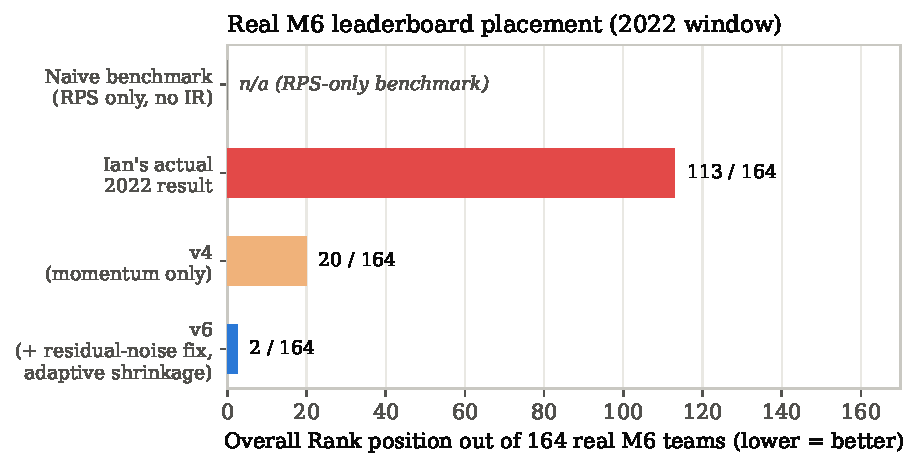
\includegraphics[width=0.7\textwidth]{figures/leaderboard_placement.pdf}
\caption{Overall Rank position (lower is better) across the naive
benchmark, the author's real result, and two intermediate versions of the
pipeline (causal momentum/reversal sign alone; final, adding the
residual-noise fix and adaptive shrinkage). Each additional fix moves
placement further toward the top of the field.}
\label{fig:leaderboard}
\end{figure}

We report this result's statistical limits plainly. With 12 monthly
observations, a one-sample $t$-test of RPS against the naive benchmark
gives $t=-1.37$, $p=0.20$; of IR against zero, $t=0.87$, $p=0.40$ ---
directionally consistent (9 of 12 periods beat the naive RPS benchmark;
8 of 12 had positive IR) but not, alone, statistically decisive. This
motivates the extension below.

\subsection{2023--2025: does it generalize out-of-sample?}

The identical walk-forward, with no reset of any adaptively learned
state, was continued through 36 further four-week periods (2023--2025)
that no design choice in this pipeline was ever informed by. Figures
\ref{fig:rps-timeseries} and \ref{fig:ir-timeseries} show all 48
resulting periods; Table \ref{tab:multiyear} reports the pooled test and
the year-by-year breakdown.

\begin{figure}[htbp]
\centering
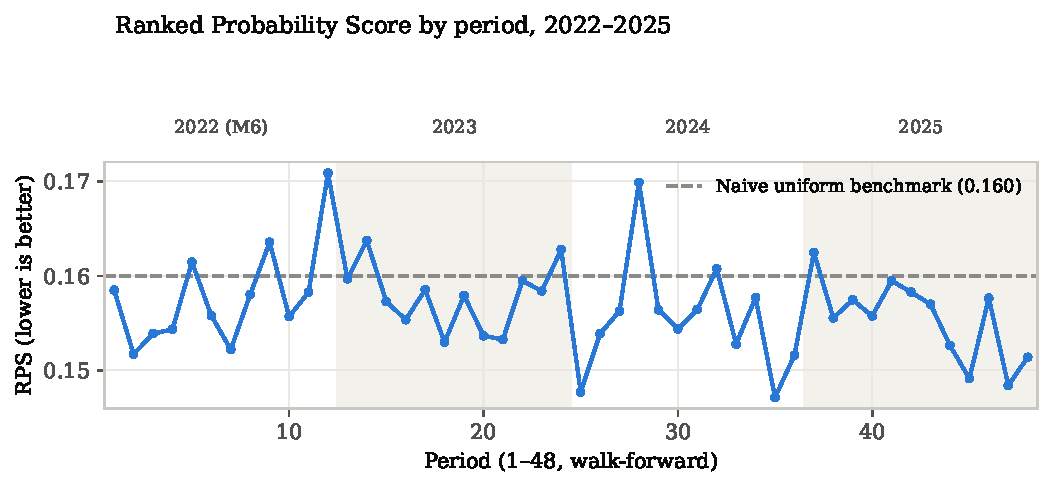
\includegraphics[width=0.95\textwidth]{figures/rps_timeseries.pdf}
\caption{RPS by period, 2022--2025. The naive benchmark (dashed) is beaten
in 40 of 48 periods (83\%).}
\label{fig:rps-timeseries}
\end{figure}

\begin{figure}[htbp]
\centering
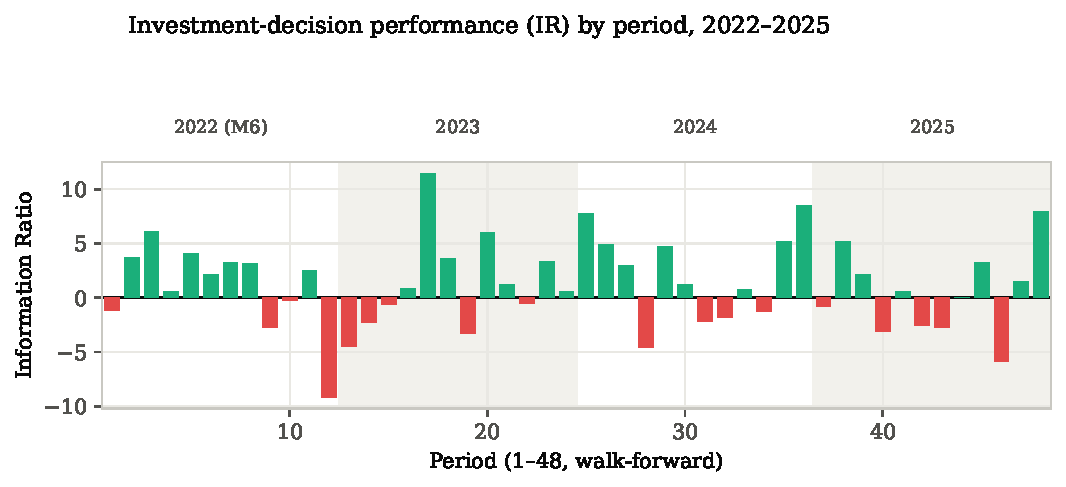
\includegraphics[width=0.95\textwidth]{figures/ir_timeseries.pdf}
\caption{Portfolio IR by period, 2022--2025. Individual months remain
volatile, as IR intrinsically is, but the pooled result across 48 periods
is positive and statistically significant.}
\label{fig:ir-timeseries}
\end{figure}

\begin{table}[htbp]
\centering
\begin{tabular}{@{}lrrrrrr@{}}
\toprule
Year & $n$ & Mean RPS & RPS $p$ & \% beat naive & Mean IR & IR $p$ \\
\midrule
2022 (M6)  & 12 & 0.1579 & 0.198 & 75\% & 1.02 & 0.404 \\
2023       & 12 & 0.1578 & 0.048 & 83\% & 1.33 & 0.317 \\
2024       & 12 & 0.1554 & 0.023 & 83\% & 2.18 & 0.096 \\
2025 (partial) & 12 & 0.1554 & 0.003 & 92\% & 0.46 & 0.690 \\
\midrule
\textbf{Pooled} & \textbf{48} & \textbf{0.1566} & \textbf{$<$0.0001} & \textbf{83\%} & \textbf{1.25} & \textbf{0.038} \\
\bottomrule
\end{tabular}
\caption{RPS and IR by year and pooled across all 48 periods.
$p$-values are one-sample $t$-tests (RPS against the naive 0.16
benchmark; IR against zero). Individual years at $n=12$ are
underpowered by design; the pooled result is the headline finding.}
\label{tab:multiyear}
\end{table}

RPS does not fade after the one year the model's design was informed by
--- if anything it is slightly better in 2024--2025 than in 2022. Figure
\ref{fig:adaptive-convergence} addresses a natural worry directly: does a
strategy with adaptively estimated parameters generalize only by
becoming unstable, chasing whatever worked most recently? Both the
momentum/reversal sign and the shrinkage blend weight instead converge
smoothly, with shrinking period-to-period variance, as more evidence
accumulates --- the behavior a well-specified expanding-window estimator
should show, not an unstable one. Diversification was re-checked across
all 48 periods to rule out concentration risk driving the IR result:
maximum single-asset weight ranged 3.6--11.4\% and top-3 concentration
10.1--20.9\% of gross exposure throughout.

\begin{figure}[htbp]
\centering
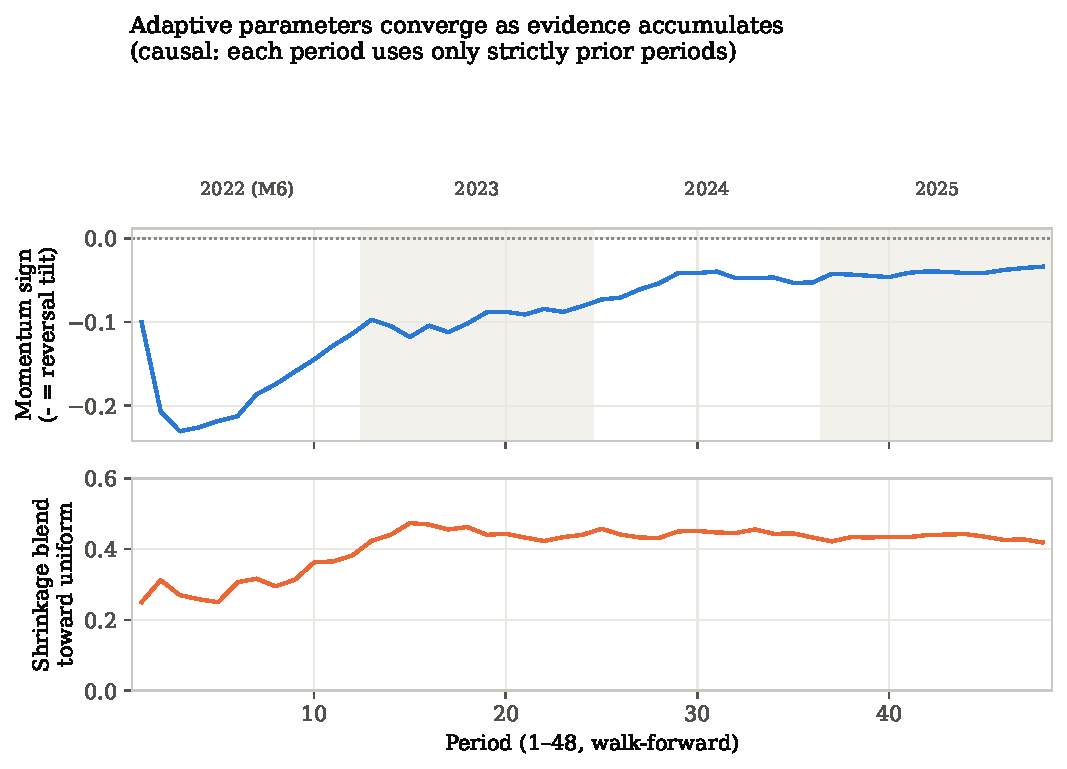
\includegraphics[width=0.75\textwidth]{figures/adaptive_convergence.pdf}
\caption{The two causally adaptive parameters (momentum/reversal sign,
top; RPS shrinkage blend, bottom) stabilize over time rather than
drifting.}
\label{fig:adaptive-convergence}
\end{figure}

\subsection{Application 2 over the same extended window}

DBMF's own total return was $+7.8\%$ in 2022, $-5.0\%$ in 2023 (a genuine
down year), $+7.2\%$ in 2024, and $+8.5\%$ in 2025 (partial). This
provides a direct test of whether Application 2's replication strategy
tracks the target's own realized performance, as one might naively
expect. It does not: Application 2's mean IR was \emph{higher} in 2023
(the year DBMF itself lost money) than in 2022, and pooled across all 48
periods its IR (mean 1.91, $t=2.64$, $p=0.011$) is, if anything, slightly
stronger than Application 1's (Figure \ref{fig:v5-v6-era}). The
resolution is that Application 2 does not statically hold the target; it
refits monthly to the target's recent return \emph{pattern} using a fresh
sparse combination of the 100 assets each period, so a target's
calendar-year total return can be negative while its short-horizon
return pattern remains learnable from the replicating universe
throughout. The real, still-standing constraint for this application is
not ``does the target keep winning,'' but ``does the target's
short-horizon return structure stay explainable by the chosen
replicating universe'' --- a condition this target and window happened to
satisfy, but not one guaranteed in general.

\begin{figure}[htbp]
\centering
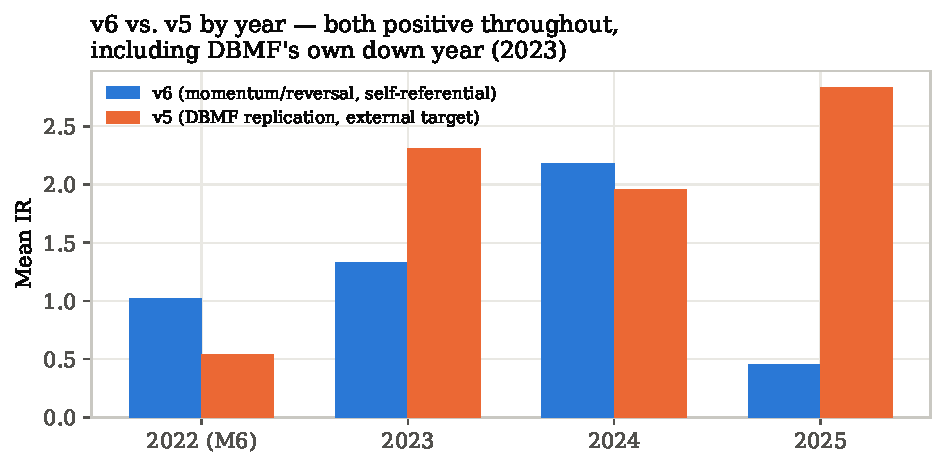
\includegraphics[width=0.72\textwidth]{figures/v5_v6_by_era.pdf}
\caption{Mean IR by year, Application 1 (self-referential forecast) vs.\
Application 2 (external-target replication). Application 2 remained
profitable even during the target's own down year (2023).}
\label{fig:v5-v6-era}
\end{figure}

% ============================================================
\section{Discussion and Limitations}
\label{sec:discussion}
% ============================================================

\textbf{Sample size.} Forty-eight monthly observations is enough to move
both headline results from directionally suggestive to statistically
significant, but not enough to rule out that a longer or differently
timed sample would look somewhat different. The per-year breakdowns are
individually underpowered by design and are reported for transparency
about year-to-year variability, not as independent confirmations.

\textbf{Data provenance.} The 2023--2025 extension uses a different price
provider than the official 2022 competition data (no official ground
truth exists to verify against post-competition), scores a 98-of-100-asset
universe (two constituents lack usable history over the full window), and
extrapolates the evaluation-window cadence forward on the assumption that
the same 28-day spacing continues, which was never externally confirmed
for the extension period.

\textbf{This is a backtest, not a live track record.} Every result here
is a retrospective evaluation of a fully specified, mechanically applied
rule, scored under a real methodology against a real external benchmark.
It does not model transaction costs, financing costs on short positions,
capacity constraints at scale, or the operational cost of actually
deploying capital against these signals. Real-time validity --- every
decision uses only information available at the time it was made --- is
a necessary condition for a backtest result to be taken seriously; it is
not a sufficient condition for it to be tradeable as-is.

\textbf{On the RPS/IR split.} This strategy's advantage is concentrated
on the investment-decision (IR) side; its RPS placement, while real and
statistically significant pooled across 48 periods, is a more modest
improvement over the naive benchmark than its IR placement is over doing
nothing. \citet{weitzenfeld2025}'s result, by contrast, was strongest
specifically on forecast accuracy. We read this as suggestive that the
two problems --- calibrated probabilistic forecasting and converting a
forecast into a good portfolio --- may reward somewhat different
modeling emphases, and see no reason the two approaches could not be
combined; we have not attempted that here.

% ============================================================
\section{Conclusion}
\label{sec:conclusion}
% ============================================================

A hierarchical spike-and-slab block-factor model, with an externally
informed prior over which correlated groups of assets are likely to
matter for a given target, produces a real, statistically significant
edge in a genuinely adversarial financial forecasting competition ---
and the edge persists, undiminished, across three further years of
out-of-sample data that had no influence on any modeling choice reported
here. We think the methodological contribution most worth taking away is
not the specific model but the discipline that made the result
trustworthy: every one of the three look-ahead leaks in Section
\ref{sec:realtime} looked entirely reasonable when first implemented, and
every one was caught only by the same mechanical, retroactively applied
question --- could this specific decision have been made with only the
information available before the fact? We think both the architecture
and that discipline generalize well beyond this one competition.

% ============================================================
\bibliographystyle{plainnat}
\bibliography{references}

\end{document}
